Un oscilador armónicose compone de una masa de 100 gramos sujeta a un muelle de constante
recuperadora de 104 dinas/cm. Se desplaza la masa una distancia de 3 cm, soltándose desde 
el reposo. Calcule:

\begin{enumerate}
    \item Frecuencia propia  $ \nu_{o}  $
    \item Periodo  $ \tau_{o}  $
    \item Energía total
    \item Velocidad máxima
\end{enumerate}

\vspace*{0.3 cm}

\begin{figure*}[h]
    \centering
    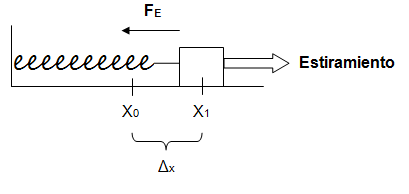
\includegraphics[scale=0.75]{masa_resorte.png}
\end{figure*}

Por la segunda ley de Newton :

\begin{align*}
    F&=ma \\
    -kx&=m \ddot{x} \\
    m \ddot{x}+kx&=0
\end{align*}

Recordemos la frecuencia angular $\omega_{o}^{2}=\frac{k}{m}$, sustituyendo:

\begin{enumerate}
    \item Frecuencia propia  $ \nu_{o}  $
\end{enumerate}

\vspace*{0.35cm}

Recordemos la frecuencia angular $\omega_{o}^{2}=\frac{k}{m}$

\vspace*{0.35cm}

Despejemos la variable $\omega_{o}$

\begin{align*}
    \omega_{o} &= \sqrt{ \frac{k}{m} }
\end{align*}

Recordando la igualdad $ \omega_{o} = 2\pi \nu_{o} $, de donde despejamos
la frecuencia propia $\nu_{o}$

\begin{align*}
    \nu_{o} &= \frac{\omega_{o}}{2\pi}
\end{align*}

Sustituyendo $\omega_{o} = \sqrt{ \frac{k}{m} }$ en la ecuación anterior.

\begin{align*}
    \nu_{o} &= \frac{ \left( \sqrt{ \frac{k}{m} } \right) }{2\pi} \\
    \nu_{o} &= \frac{ 1 }{2\pi} \sqrt{ \frac{k}{m} }
\end{align*}

Sustituyendo en la ecuación anterior:

\begin{align*}
    \nu_{o} &= \frac{ 1 }{2\pi} \sqrt{\frac{( 10^{4} dinas/cm )}{(100 g)}}\\
    \nu_{o} &= 1.6 \frac{1}{s}
\end{align*}

$\therefore$ La frecuencia propia es  $ \nu_{o} = 1.6 \frac{1}{s}$

\vspace*{0.4cm}

b. Periodo  $ \tau_{o}  $

Anteriormente llegamos a la ecuación

\begin{equation*}
    \nu_{o} = \frac{ 1 }{2\pi} \sqrt{ \frac{k}{m} }
\end{equation*}

Recordemos que $\nu_{o}=\frac{1}{\tau_{o}} $, vamos a realizar esta sustitución en la ecuación
anterior:

\begin{align*}
    \frac{1}{\tau_{o}} &= \frac{ 1 }{2\pi} \sqrt{ \frac{k}{m} } \\
                       &= \frac{ \sqrt{k} }{ 2\pi \sqrt{m} }
\end{align*}

Despejamos para el periodo $\tau_{o}$:

\begin{align*}
    \tau_{o}    &= \frac{ 1 }{2\pi} \sqrt{ \frac{k}{m} } \\
                &= \frac{ 2\pi \sqrt{m}  }{ \sqrt{k} } \\
                &= 2\pi \sqrt{ \frac{m}{k} }
\end{align*}

Sustituyendo en la ecuación anterior:

\begin{align*}
    \tau_{o}&= 2\pi \sqrt{ \frac{( 100 g )}{( 10^{4} dinas/cm )} }\\
    \nu_{o} &= 0.62 s
\end{align*}

$\therefore$ El periodo es  $ \tau_{o} = 0.63 $ s

c. Energía total

\vspace*{0.5cm}

Como la energía total es la suma de la energía potencial y la energía cinética, primero
buscaremos expresiones para la velocidad y la posición.

Recordemos la ecuación diferencial del sistema

\begin{equation*}
    m \ddot{x}+kx=0
\end{equation*}

Observación: $ m \ddot{x}+kx=0 $ es una ecuación diferencial lineal
homogénea de orden dos con coeficientes constantes.

\vspace*{0.35cm}

Y de la redacción del problema identificamos las siguientes condiciones iniciales:

\begin{align*}
    x(0) = x_{o} = 3cm \\
    \dot{x} (0) = 0
\end{align*}

Observación: Tenemos condiciones iniciales en $t=0$ por tanto podemos
usar la transformada de Laplace para resolver la ecuación diferencial.

\begin{align*}
    \Laplace \left\{ m \ddot{x}+kx \right\} &= \Laplace \left\{ 0 \right\}
\end{align*}

Recordemos que $ \Laplace \left\{ 0 \right\} = 0 $

\begin{align*}
    \Laplace \left\{ m \ddot{x} \right\} + \Laplace \left\{ kx \right\} &= 0 \\
    m \Laplace \left\{ \ddot{x} \right\} + k \Laplace \left\{x  \right\} &= 0
\end{align*}

Sea $\Laplace \{ x(t) \} = X(s)$ y recordando que $ x(0)= x_{o} = 3cm $ y $ = \dot{x} (0)=0$ 

\begin{itemize}
    \item En $m \Laplace \left\{ \ddot{x} \right\} $: 
\end{itemize}

\begin{align*}
    m \Laplace \left\{ \ddot{x} \right\} &= m \left( s^{2}X(s) -sx(0) - \dot{x}(0) \right) \\
                                         &= m \left( s^{2}X(s) -sx_{o} - 0 \right) \\
                                         &= m s^{2}X(s) -msx_{o}
\end{align*}

\begin{itemize}
    \item En $ k \Laplace \left\{ x \right\} $: 
\end{itemize}

\begin{align*}
    k \Laplace \left\{ x \right\} &= k X(s)
\end{align*}

Sustituyemos las anteriores igualdades en la ecuación diferencial:

\begin{align*}
    m s^{2}X(s) -msx_{o} + k X(s) = 0 
\end{align*}

Ahora despejamos para $X(s)$ :

\begin{align*}
    m s^{2}X(s) -msx_{o} + k X(s) = 0 \\
    m s^{2}X(s) + k X(s) = mx_{o}s 
\end{align*}

\begin{align*}
    X(s) \left( m s^{2} + k \right) &= mx_{o}s \\
    X(s)  &= \frac{mx_{o}s}{m s^{2}+k} \\
    X(s)  &= \frac{mx_{o}s}{ m \left( s^{2} + \frac{k}{m} \right) } \\
    X(s)  &= \frac{x_{o}s}{  s^{2} + \frac{k}{m}  }
\end{align*}

Ahora aplicamos la transformada inversa de Laplace en ambos lados de la ecuación:

%   \Laplace^{-1} \{  \}

\begin{align*}
    \Laplace^{-1} \{ X(s) \} &= \Laplace^{-1} \left\{\frac{x_{o}s}{  s^{2} + \frac{k}{m}} \right\} \\
                             &= x_{o} \Laplace^{1} \left\{\frac{s}{ s^{2} + \frac{k}{m} }\right\} 
\end{align*}

Como  $ \Laplace^{-1} \left\{\frac{s}{s^{2}+k^{2}}\right\} = Cos(kt) $

\vspace*{0.4cm}

\begin{equation*}
    \Rightarrow \Laplace \left\{ \frac{s}{ s^{2} + \frac{k}{m}  } \right\} = Cos \left( \sqrt{ \frac{k}{m} } t \right)
\end{equation*}

\vspace*{0.4cm}

Tambien sabemos que $ \Laplace^{-1} \left\{X(s)\right\} = x(t) $

\vspace*{0.35cm}

Hacemos las sustituciones de las transformadas inversas de Laplace:

\begin{equation*}
    \therefore x(t) = x_{o} Cos \left( \sqrt{ \frac{k}{m} } t \right)
\end{equation*}

Ahora para determinar $\dot{x} (t)$ derivamos a $q(t)$ :

\begin{align*}
    x(t) &= x_{o} Cos \left( \sqrt{ \frac{k}{m} } t \right) \\
    \therefore \dot{x}(t) &= - \sqrt{ \frac{k}{m} } x_{o} Sen \left(  \sqrt{ \frac{k}{m} } t \right)
\end{align*}

Recordando que $T=\frac{1}{2} m \dot{x}^{2}$

\begin{equation*}
    T=\frac{1}{2} m \frac{k}{m} x_{o}^{2} Sen^{2} \left(  \sqrt{ \frac{k}{m} } t \right)
\end{equation*}

Recordando que $V=\frac{1}{2} kx^{2}$

\begin{equation*}
    T=\frac{1}{2} k x_{o} Cos \left( \sqrt{ \frac{k}{m} } t \right)
\end{equation*}

Y como la energía mecánica está dada por $E=T+V$

\begin{align*}
    E   &=T+V \\
        &=\frac{1}{2} m \frac{k}{m} x_{o}^{2} Sen^{2} \left(  \sqrt{ \frac{k}{m} } t \right) 
           + \frac{1}{2} k x_{o}^{2} Cos^{2} \left( \sqrt{ \frac{k}{m} } t \right)
\end{align*}

En ese sistema solo actúan fuerzas conservativas, por tanto la energía se conserva.

Evaluemos la energía en el tiempo $t=0$ :

\begin{align*}
    E(0)&=\frac{1}{2} (100 g) \frac{( 10^{4} dinas/cm )}{m} (3cm)^{2} Sen^{2} \left(  \sqrt{ \frac{( 10^{4} dinas/cm )}{(100 g)} } (0s) \right) \\
        &\hspace{0.23cm}+ \frac{1}{2} ( 10^{4} dinas/cm ) (3cm)^{2} Cos^{2} \left( \sqrt{ \frac{( 10^{4} dinas/cm )}{(100 g)} } (0s) \right) \\
        &= \frac{1}{2} ( 10^{4} dinas/cm ) (3cm)^{2} \\
        &= 45000 ergios
\end{align*}

$\therefore$ La energía total del sistema es de 45000 ergios


d. Velocidad máxima

Retomemos la ecuación de la velocidad que encontramos:

\begin{equation*}
    \dot{x}(t) = - \sqrt{ \frac{k}{m} } x_{o} Sen \left(  \sqrt{ \frac{k}{m} } t \right)
\end{equation*}

Expresemos el módulo de la velocidad:

\begin{align*}
    \left\lVert \dot{x}(t) \right\rVert &= \sqrt{ \left( - \sqrt{ \frac{k}{m} } x_{o} Sen \left(  \sqrt{ \frac{k}{m} } t \right) \right)^{2} } \\
    \left\lVert \dot{x}(t) \right\rVert &= \sqrt{ \frac{k}{m} } x_{o} Sen \left(  \sqrt{ \frac{k}{m} } t \right)
\end{align*}

Esta expresión alcanza su máximo cuando: $ Sen \left(  \sqrt{ \frac{k}{m} } t \right) = 1 $

\begin{equation*}
    \left\lVert \dot{x}(t) \right\rVert_{max} = \sqrt{ \frac{k}{m} } x_{o}
\end{equation*}

Sustituyendo en la ecuación anterior:

\begin{align*}
    \left\lVert \dot{x}(t) \right\rVert_{max} &= \sqrt{ \frac{( 10^{4} dinas/cm )}{(100 g)} } (3cm) \\
                                              &= 30 \frac{cm}{s}  
\end{align*}

$\therefore$ La velocidad máxima es de 30 $\frac{cm}{s}$

\vspace*{0.5cm}

\textbf{Por lo tanto:}

\begin{enumerate}
    \item \textbf{La frecuencia propia es  $ \nu_{o} = 1.6 $ $\frac{1}{s}$}
    \item \textbf{El periodo es  $ \tau_{o} = 0.63 $ s}
    \item \textbf{La energía total del sistema es de 45000 ergios}
    \item \textbf{La velocidad máxima es de 30 $\frac{cm}{s}$}
\end{enumerate}